На рисунке схематически показано, что происходит с воздухом в салоне самолета за одну минуту:
\begin{itemize}
\item Поступает объем воздуха без пыли, равный $U$. В нижней части схемы этому объему соответствует левый кусок.
\item Такой же объем $U$ грязного воздуха выходит из салона самолета. Это следует из того, что количество воздуха в салоне сохраняется. Очевидно, что количество пылинок, которые покинули самолет, равняется $N_{out} = C U$. Кажется, что грязи должно стать меньше, но:
\item в воздух поступает $N = N_P + N_F$ пылинок, где мы обозначили как $N_P$ количество пылинок от людей, и $N_F$ количество пылинок с полу.
\end{itemize}

\begin{center}
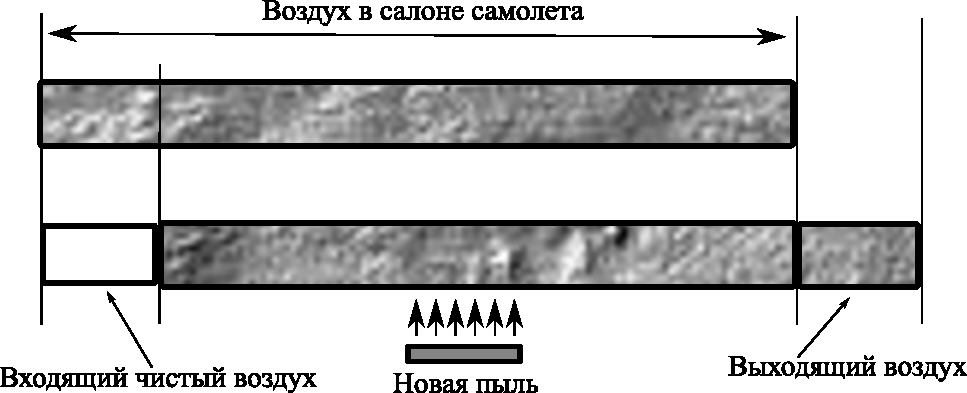
\includegraphics[scale=0.7]{Solutions/pic/s-spb19-07-4-f1.pdf}
\end{center}

Так как количество пылинок в салоне со временем не меняется (концентрация и объем салона постоянны), значит число поступающих и выходящих пылинок равно друг другу:
\begin{equation}
C U = N_{out} = N_P + N_F \mbox{ . } \label{eq:spb19_07_04_1}
\end{equation} 
Если увеличить наддув воздуха кондиционером, то правая часть уравнения не изменится. Значит при увеличении $U$ в два раза, концентрация уменьшится в два раза. Исходя из условия можно записать:
\begin{equation}
C - \frac{C}{2} = \Delta C_1 = 100 \mbox{ (} 1/\mbox{см}^{3} \mbox{)  или }  C = 200 \mbox{ (}1/\mbox{см}^{3} \mbox{ )} \mbox{ . }
\end{equation}
Рассмотрим далее второй случай: когда наддув остается неизменным, а количество пассажиров удваивается. Во-первых, величина $N_P$ увеличится два раза. Во-вторых, концентрация увеличится от значения $C$ до $C+\Delta C_2$, или в $\frac{3}{2}$ раза. Так же из условия следует, что $N_F$ не измениться. Этих данных достаточно, чтобы найти все неизвестные. Например, составим систему уравнений, которая описывает приведенные условия:
\begin{eqnarray}
C U = N_P + N_F \\
\frac{3}{2} C U = 2 N_P + N_F \label{eq:spb19_07_04_2} \mbox{ . }
\end{eqnarray}
Из этих двух уравнений можно получить, что:
\begin{equation}
N_F = \frac{1}{2} C U \mbox{ . }
\end{equation}
Величина $C U$ это, фактически, количество частиц, находящихся в объеме 15 м$^3$. Таким образом, $N_F = 1500 \cdot 10^6$, где мы учли, что 1 м$^3$ = 10$^6$ см$^3$. За одну секунду с пола улетает в 60 раз меньше частиц, т.е. $N_F/60$.


\underline{\textbf{Ответ:}} За одну секунду с пола улетает $25 \cdot 10^6$ частиц пыли.

\begin{itemize}
\item \textbf{1 балл} --- Обнаружено понимание факта, что ''добавленный'' чистый воздух вытесняет запыленный. При этом уход частиц пыли компенсируется приходом пыли от людей и с пола. В идеале, должно быть написано уравнение типа (\ref{eq:spb19_07_04_1}), но это необязательно.

\item \textbf{1 балл} --- Правильно рассмотрен случай увеличения $U$ в два раза. Вычислено значение концентрации $C = 200$~см$^{-3}$.

\item \textbf{1 балл} --- Правильно рассмотрен случай увеличения числа пассажиров в два раза. Записано уравнение типа (\ref{eq:spb19_07_04_2}). Или словами выражены утверждения про $\frac{3}{2}$ и $2 N_P$.

\item \textbf{1 балл} --- Правильный численный ответ.

\end{itemize}


